%!TEX encoding = UTF-8 Unicode
%!TEX root = ../compendium1.tex

\chapter{Fixa buggar}\label{appendix:debug}

\begin{figure}[H]
\centering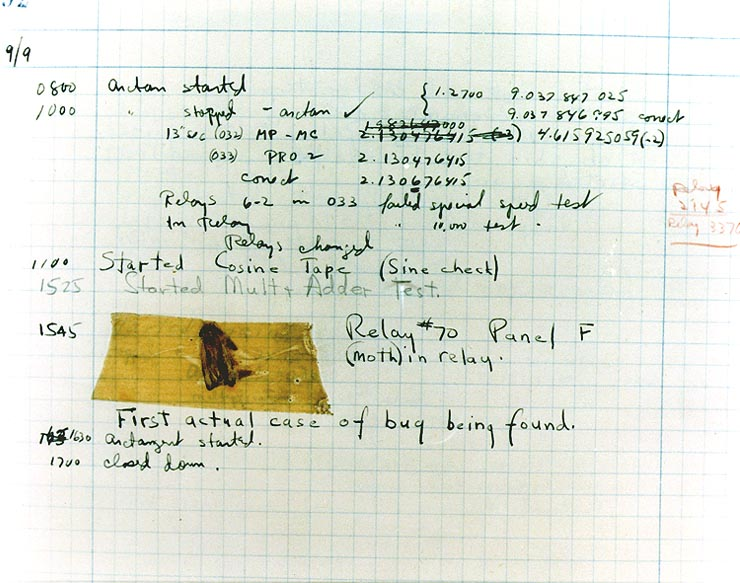
\includegraphics[width=0.85\textwidth]{../img/bug}

\caption{Den första dokumenterade buggen hittades 9 september 1947 i en Mark II Aiken Relay Calculator av Grace Hopper.\protect\footnotemark}

\end{figure}\footnotetext{\href{https://commons.wikimedia.org/w/index.php?curid=165211}{commons.wikimedia.org/w/index.php?curid=165211} Courtesy of the Naval Surface Warfare Center, Dahlgren, VA., 1988. - U.S. Naval Historical Center Online Library Photograph NH 96566-KN, Public Domain.   }


\section{Vad är en bugg?}

En bugg, även kallad lus \Eng{bug}, är en felaktighet som kan göra så att ett program inte beter sig som det är tänkt, och kan innebära oönskad utdata, att programmet kraschar, eller till och med ond bråd död.\footnote{\href{https://www.theguardian.com/technology/2016/jul/01/tesla-driver-killed-autopilot-self-driving-car-harry-potter}{www.theguardian.com/technology/2016/jul/01/tesla-driver-killed-autopilot-self-driving-car-harry-potter}}

Ursprunget till ordets användning i programmeringssammanhang är något oklar, men kan härledas till engelskans \emph{bug} som betyder insekt eller småkryp. 
Man brukar berätta att vid en felsökning av ett program som körde i en tidig dator byggd med  elektromekaniska reläer, uppdagades en död nattfjäril ihjälklämd mellan drivankaret och spolen i ett relä, som orsakade att programmet inte kunde exekveras korrekt. 



\subsection{Olika sorters fel}

När man ska lära sig mer om fel i programvarubaserade system, och hur de kan åtgärdas, är det viktigt att noga skilja på \textbf{misstag} \Eng{mistake}, \textbf{felorsak} \Eng{fault} och \textbf{felyttring} \Eng{failure}. 
Med ''misstag'' menar vi här ett fel som begås av människor (utvecklare, systemadministratörer, operatörer, användare, etc.) medan de skapar och använder ett programvarusystem. 

Det kan bli fel i olika delar av processen: 
\begin{itemize}
\item \textbf{Kravfel} uppstår medan man tänker ut vad systemet ska göra och då misstar sig angående  användarnas behov och önskemål.
\item \textbf{Designfel} uppkommer när man utformar systemets struktur på ett dåligt sätt.
\item \textbf{Implementeringsfel} begås när man programmerar och skriver felaktiga kodrader. 
\item \textbf{Testfel} förekommer vid provkörning av systemet då testkoden är felaktig och därför ger falskt alarm om ''fel'', trots att beteendet egentligen är korrekt.  
\item \textbf{Operatörsfel} sker när systemet lämnas över till de, som ska installera och köra systemet i skarp produktion, och där systemdriften \Eng{operations, ''ops''} sköts på ett sätt som får problematiska konsekvenser.
\item \textbf{Användarfel} händer då användarna ger felaktig indata, eventuellt i strid med riktlinjerna för hur systemet ska användas, som systemet inte klarar att hantera korrekt, varpå mer eller mindre allvarliga felbeteenden hos systemet följer.
\end{itemize} 
I olika delar av utvecklingsprocessen kan alltså misstag begås som, antingen omedelbart, eller någon gång i framtiden, kan orsaka fel. Men det är inte säkert att ett fel någonsin kommer att märkas. Kanske kommer de felaktiga kodraderna, som \emph{skulle} kunna orsaka ett fel, aldrig att exekveras. Eller så kommer ingen användare att någonsin vilja använda systemet så som stipuleras av (onödiga) krav. Det är alltså först när fel \emph{yttrar} sig vid exekvering som misstag märks.

Fel kan också kategoriseras utifrån \emph{hur} de upptäcks i utvecklingsprocessen. Man brukar skilja på fel upptäckta vid granskning, kompileringsfel och exekveringsfel, som diskuteras nedan:
\begin{itemize}
\item Fel upptäckta vid \textbf{granskning}. Ett effektivt sätt att upptäcka fel är att människor noga läser igenom sin egen, och andras kod och försöker leta efter möjliga problem och brister. Man blir ofta ''hemmablind'' när det gäller ens egen kod. Därför kan någon annans, oberoende granskning med ''nya, friska'' ögon vara mycket fruktbar.  I samband med kodgranskning kan man med fördel försöka bedöma  huruvida koden är lätt att läsa, lätt att ändra i eller om koden har andra viktiga kvaliteter som har betydelse för den framtida utvecklingen av koden. Ofta hittar man vid granskning även enkla programmeringsmisstag, så som felaktiga villkor och loop-räknare som inte räknas upp på rätt sätt etc.
  
\item \textbf{Kompileringsfel} uppkommer under kompilering och upptäcks tack vare kontroller som sker av  kompilatorn. 

Vid kompileringsfel får man också ofta av kompilatorn reda på \emph{var} i koden det är fel och \emph{varför} det är fel, så att sökandet efter felorsaken och åtgärdandet av misstaget underlättas. Men ibland är felmeddelandet från kompilatorn missvisande och pekar på helt fel ställe i koden, så det gäller att inte alltid lita blint på det kompilatorn skriver. Dessutom är felmeddelanden från kompilatorn ofta uttryckta i termer av språkets syntaktiska och semantiska regler och det tar tid att lära sig tolka kompilatorers felmeddelanden. Att skapa kompilatorer som ger bra felmeddelande är ett svårt problem som studeras inom den datavetenskapliga disciplinen \textit{kompilatorteknik}, vilken du kan lära mer om i kurser på avancerad nivå.

Olika programmeringsspråk erbjuder olika stora möjligheter att göra kontroller vid kompileringstid. En kompilator för ett språk med ett avancerat typsystem, som till exempel Scala, ger förhållandevis stora möjligheter att identifiera fel redan under kompileringen, medan man med ett språk med ett svagare typsystem, till exempel Javascript, får förlita sig på prestandahämmande kontroller som kompilatorn genererar i maskinkoden eller som du själv väljer att lägga in i källkoden för säkerhets skull. 
  
\item \textbf{Exekveringsfel}, även kallat körtidsfel \Eng{runtime error}, sker medan programmet körs. Det kan krävas viss, specifik indata under specifika exekveringsomständigheter (en viss processor, en viss minnesstorlek, en viss nätverkskapacitet etc.) för att ett exekveringsfel ska yttra sig. När ett exekveringsfel väl yttrar sig, kan olika saker hända:

\begin{itemize}

\item \textbf{Exekveringen ger oönskat resultat.} Det är inte säkert att ett exekveringsfel avbryter exekveringen; det är vanligt att felet ''bara'' resulterar i inkorrekt utdata eller på annat sätt ger dålig kvalitet. För att upptäcka detta innan systemet sätts i drift, är det allmän praxis att man skriver noga uttänkta \textbf{testfall} och analyserar \textbf{testresultat} från exekveringen av  testfallen i detalj genom att undersöka utdata i jämförelse med önskat resultat eller med vad som anses vara en tillräckligt hög kvalitetsnivå.

\item \textbf{Exekveringen hänger sig} \Eng{hang}. Ibland yttrar sig fel genom att inget alls ser ut att hända under exekveringen, vilket kan beror på t.ex.:  
\begin{itemize}[nolistsep]
\item en \textbf{oändlig loop}, som aldrig blir färdig, 
\item att det går \textbf{väldigt långsamt} eftersom bearbetningen av indata tar orimligt lång tid,
\item att programmet \textbf{väntar på indata} som aldrig kommer,
\item att olika jämlöpande delar av programmet väntar på varandra så att ett \textbf{dödläge} \Eng{deadlock} uppstår. 
\end{itemize}

När exekveringen hänger sig och man inte orkar vänta längre på att något ska hända, är det bara att brutalt avbryta exekveringen genom något lämpligt kommando som erbjuds i din körmiljö.\footnote{\texttt{kill -9} $<$pid$>$, Ctrl+C, Ctrl+Shift+C, Ctrl+Z eller något annat beroende på körmiljö.} I värsta fall får man stänga av strömmen.

\item \textbf{Exekveringen kraschar} \Eng{crash}. Ibland blir det ett plötsligt tvärstopp och exekveringen avbryts med ett körtidsfelmeddelande. Detta kan bero på t.ex.:
\begin{itemize}[nolistsep]
\item att \textbf{minnet är slut}, antingen är det parameterminnet för funktionsanrop \Eng{stack memory} som tagit slut eller så är minnet för allokering av objekt som skapas under programmets gång \Eng{heap memory} fullt,
 
\item misstaget att försöka referera en \textbf{null-referens} som inte refererar till något objekt, utan har värdet \code{null}, vilket resulterar i  \textit{null pointer exceeption},

\item att ett s.k. \textbf{undantag} har ''kastats'' \Eng{throw exception} genom att den som skrivit programmet medvetet kodat så att ett oönskat feltillstånd \emph{ska} orsaka en krasch, om inte undantaget ''fångas'' \Eng{catch} och hanteras av omgivande kod. 
\end{itemize}

När systemet kraschar får man en lista med den aktuella kedjan av funktionsanrop i en \textbf{stackspårning} \Eng{stack trace}. Man kan också begära en utskrift av hela innehållet i minnet vid kraschen \Eng{memory dump}, men en sådan kan vara svår att tolka.

\end{itemize}

\end{itemize}

När systemet ger oönskade resultat, hänger sig eller kraschar, får man försöka återskapa exekveringsfelet i en omkörning och, med hjälp av instrumentering eller en debugger, försöka lista ut vad som händer precis \emph{innan} exekveringsfelet uppstår, se  avsnitt \ref{section:debugging}.

I kursen \textit{Programvarutestning} \Eng{Software Testing} lär du dig mer om systematiska metoder för att testa system så att fel kan förebyggas, identifieras och åtgärdas.

\subsubsection{Bugg eller feature?} 

När ett (eventuellt) fel upptäcks, kan det vara på sin plats att först ställa sig några grundläggande  frågor:

\begin{itemize}
\item Är detta verkligen ett ''fel'' eller är det egentligen ett avsett beteende? Det är inte alltid självklart om det är en bugg eller en medvetet skapad systemegenskap/funktion \Eng{feature}.

\item Är det kanske testfallet som har felaktig testkod, medan koden som testas egentligen fungerar alldeles utmärkt? Sådan problem kan vara speciellt svåra att lösa, då man ofta letar på fel ställe efter orsaken.

\item Om buggen rör någon kvalitetsegenskap hos systemet kan man fråga sig: Var går egentligen gränsen för ''fel''? Är detta bra nog givet vad det kostar att förbättra kvaliteten? Kvalitetskrav berör egenskaper hos ett program som kan uttryckas på en glidande skala, där något kan vara mer eller mindre \emph{bra} eller \emph{dåligt} ur olika synvinklar. Sådana krav leder ofta till viktiga men svåra avvägningsbeslut under design och implementation. Dessutom kan testresultat bli svårbedömda och det kan finnas olika åsikter om huruvida ett eventuellt fel är en bugg eller inte.

Här är några exempel på kvalitetskrav:
\begin{itemize}
\item \textbf{Prestandakrav} \Eng{performance requirements} avser hur snabbt och effektivt programmet ska arbeta under olika omständigheter.
 
\item \textbf{Kapacitetskrav} \Eng{capacity requirements} avser hur mycket data systemet ska klara av under olika omständigheter.

\item \textbf{Användbarhetskrav}\footnote{\href{https://sv.wikipedia.org/wiki/Anv\%C3\%A4ndbarhet}{sv.wikipedia.org/wiki/Användbarhet}} \Eng{usability requirements} avser krav på hur lättanvänt systemet ska vara för en given användarkategori. 
\end{itemize} 

\end{itemize}

I kursen \textit{Kravhantering} \Eng{Sofware Requirements Engineering} lär du dig mer om att identifiera, specificera och följa upp kvalitetskrav.

\subsubsection{Felärendehanteringsverktyg} 

Det är allmän praxis i industriell systemutveckling att använda sig av ett felärendehanteringsverktyg \Eng{issue tracker} så att samarbetande utvecklare får stöd i att hålla reda på alla uppkomna fel och problem \Eng{issue}. Många av de populära kodlagringsplatserna som finns på nätet, så som GitLab, GitHub och BitBucket (se avsnitt \ref{section:code-hosting}), erbjuder felärendehanteringsfunktioner. Dessa kan till exempel vara:
\begin{itemize}
\item hantering och sammanställning av alla olika ärendetillstånd, så att man kan se vilka issues som är i tillstånden \textit{Open} eller \textit{Closed},
\item tillording av ärende till specifika personer som ska åtgärda problemet,
\item gradering av ärende i olika allvarlighetsgrader,
\item meddelandegenerering till inblandade personer när ett ärende kommenteras eller ändrar tillstånd.
\end{itemize}


\section{Att förebygga fel}

Även om det nästan är oundvikligt att låta buggar slinka in i koden allteftersom den blir mer och mer komplex, är det ändå viktigt att lägga stor möda vid att försöka undvika att så sker. Det är ofta mycket bättre investerad tid att jobba med buggförebyggande åtgärder medan du skapar koden, än att jaga buggar som skulle kunna ha undvikts med allmän noggrannhet och stramare disciplin i kodningen. Nedan sammanfattas några åtgärder som kan hjälpa till att minska mängden fel.

\begin{itemize}
\item \textbf{Skapa begriplig kod}. Grunden för att undvika buggar är anstränga sig att skriva begriplig kod som är lätt att läsa. Detta är en ständig kamp; kodens komplexitet växer för varje tillägg och med jämna mellanrum behövs omstruktureringar \Eng{refactoring} för att bibehålla en god struktur som underlättar begripligheten och gör utvidgningar lättare. 
%En integrerad utvecklingsmijlö erbjuder stöd för att omstrukturera kod  med bibehållen korrekthet. 

\item \textbf{Tänk ut bra namn}. En viktig pusselbit för att skapa begriplig kod är att tänka ut bra namn. Detta kan vara förvånansvärt svårt och kan kräva mycket diskussioner och tankemöda. 
%I själva namnet ligger ofta en stor del av möjligheten för en abstraktion du skapat att nå ut till dina medutvecklare med rätt associationer, som genom sitt namn antingen kan skapa härligt läsbar programtext, eller oerhört svårigenomtränglig gröt där namnen snarast upplevs som desinformation. 
Om du inser att ett namn är illa valt är det förmodligen värt jobbet att omstrukturera koden och införa ett bättre namn, speciellt om andra ännu inte vant sig alltför mycket vid begreppet. 
%Ibland när ett namn ''kliar'' beror det på att själva abstraktionen är feltänkt och behöver tänkas om. 
%En integrerad utvecklingsmiljö erbjuder stöd för att byta namn på precis rätt ställe, med hänsyn till synlighet och blockstruktur. 

\item \textbf{Kontrollera parametrar och variabler}. Ofta känner man till vilka villkor som måste gälla för olika variablers värden. Till exempel vet man ofta att en viss funktionsparameter av heltalstyp inte får vara negativ. Då kan man säkerställa detta genom att lägga in kontroller av att villkoret är uppfyllt. Vid villkor som gäller parametrar, brukar man i Scala anropa \code{require}, till exempel: \code{require(x >= 0, "x must be positive")}. Det finns också en metod \code{assert} som fungerar på samma vis\footnote{\href{http://stackoverflow.com/questions/26140757/what-to-choose-between-require-and-assert-in-scala}{stackoverflow.com/questions/26140757/what-to-choose-between-require-and-assert-in-scala}}; medan \code{require} används för att kontrollerar parametrar, brukar \code{assert} användas för att kontrollera generella villkor som ska gälla, till exempel \code{assert(x + y > n, "overflow")}.  Fördelen med att lägga in kontroller av villkor är att villkorsbrott upptäcks direkt och felsökningen blir lättare. 

\item \textbf{Kontrollera typer}. Med \textit{typannoteringar} får du hjälp av kompilatorn att kontrollera dina hypoteser om vilka typer olika värden har. I Scala kan du nästan var du vill i ett uttryck lägga till ett kolon och en typ för att begära att kompilatorn kontrollerar typen. Till exempel kan du skriva \code{(xs + f(42)) : Set[Int]} för att säkerställa att uttrycket \code{xs + f(42)} verkligen ger en mängd med heltal. Även om du sällan i Scala behöver ange typer explicit, tack vare kompilatorns typinferens, bidrar det till läsbarheten och skapar säkrare kod om du på lämpliga ställen ändå anger de typer som du förväntar dig, speciellt vid i komplicerade uttryck eller långa kedjor av metodanrop, och när metoders returtyper inte är uppenbara. Dessutom kan kompilatorn ibland undvika att gå vilse i speciellt svåra typhärledningar, om du hjälper den på traven med explicita typannoteringar.

\item \textbf{Hantera saknade värden}. Det är mycket vanligt att man måste hantera situationer där ett värde saknas, inte kan beräknas, eller inte finns tillgängligt av andra orsaker. Man kan hålla reda på att ett värde saknas genom att representera detta med speciella värden, t.ex. \code{-1} eller \code{null}. Men den strategin leder mycket lätt till buggar, då man lätt glömmer att på andra ställen i koden kontrollera dessa speciella värden. Med sådana speciella värden får man heller ingen hjälp av kompilatorn att upptäcka att man missat att ta hand om dem. Om man istället hanterar eventuellt saknade värden med \code{Option} (se kapitel \ref{chapter:W10}), så får man hjälp vid kompileringstid och slipper exekveringsfel och besvärlig felsökning. Det blir dessutom väldigt tydligt för alla som läser din kod, inklusive du själv, att ett värde kan saknas.
 
\item \textbf{Hantera undantag}. När undantag uppstår, t.ex. att en fil inte kan läsas eller det blir division med noll, avbryts exekveringen och programmets användare kan inte använda programmet längre, vilket i värsta fall kan få ödesdigra konsekvenser. Därför vill man hantera undantagssituationer på ett sådant sätt att programmet blir robust och inte kraschar. Detta kan man med fördel göra genom att kapsla in undantaget i ett värde av typen \code{Try}, se kapitel \ref{chapter:W10}. I likhet med \code{Option} för saknade värden, blir det tydligt i koden att ett värde av typen \code{Try} kan innebära ett lyckat resultat (\code{Success}), eller så fallerar beräkningen (\code{Failure}) med en inkapslad, förhindrad krasch. 

\item \textbf{Granska kod}. Det är allmän praxis i industriell programvaruutveckling att göra kodgranskningar, vid vilka en grupp människor noga studerar någon annans kod och ger kommentarer och identifierar potentiella problem. Ofta har man en checklista att utgå ifrån medan man läser koden, som innehåller punkter man vill kontrollera speciellt, t.ex. begriplighet, namngivning, kontroller av parametrar, hantering av saknade värden och undantag, etc. Många organisationer har en överenskommen kodningsstandard med riktlinjer för kodens utseende och stil som alla ska följa om inte speciella skäl finns. Att sådana stilriktlinjer följs kan kontrolleras genom granskningar. Det finns också verktygsstöd för att göra sådana kontroller. Ett exempel på kodningsriktlinjer för Scala finns på den officiella dokumentationssajten\footnote{\url{http://docs.scala-lang.org/style/scaladoc.html}}. 

\item \textbf{Testa kod}. Det är allmän praxis i industriell programvaruutveckling att genomföra tester på flera olika nivåer. Man kombinerar ofta \textbf{enhetstest} \Eng{unit test} av enskilda delar av koden, med \textbf{funktionstest} \Eng{feature test} för att se så att indata i en tänkt användningssituation ger önskat resultat, och \textbf{systemtest} \Eng{system test} för att se att alla delar fungerar tillsammans under realistiska omständigheter. 

\item \textbf{Lär av användarnas upplevelser}. När koden sätts i produktion finns möjlighet att lära sig genom återkoppling från användare. Hur systemet används och hur användarna upplever det att använda systemet är mycket viktig information när man ska besluta om hu koden bäst ska utveckla vidare. Från användarna kan man få reda på både okända buggar och få briljanta idéer till nya värdefulla funktioner. En mjukvaruutvecklande organisations innovationsförmåga beror i stor utsträckning på dess förmåga att kontinuerligt leverera kod som får allt fler funktioner som användarna gillar, utan att för många irriterande eller ödesdigra buggar.

\end{itemize}



\section{Vad är debugging?}

När en felyttring identifierats, t.ex. genom testning eller slutanvändare rapporterar om problem, vidtar sökandet efter den bakomliggande felorsaken, så att vi förstår \emph{varför} det blev fel och sedan kan \emph{åtgärda} misstaget. Denna process kallas \textbf{avlusning} \Eng{debugging}.




\subsection{Hur hittas felorsaken?}

Första steget i avlusningsprocessen är att hitta den bakomliggande felorsaken. Detta kan vara mycket svårt, speciellt om systemet är stort och komplicerat.

När du stirrar dig blind på koden utan att hitta felorsaken, kan det bero på att du har en felaktig hypotes om vad koden egentligen gör. Du är övertygad om att en viss sak händer, men \emph{egentligen} är det \emph{inte} det du \emph{tror} händer som \emph{verkligen} händer. Exempelvis kanske du antar att en räknare räknas upp i en loop, men i själva verket saknas uppräkningen. Om du oreflekterat accepterar ditt felaktiga antagande, är det stor risk att du letar på fel ställe i koden.

Följande åtgärder är ofta lämpliga när man jagar buggar:


\begin{itemize}

\item \textbf{Återskapa buggen med ett minimalt testfall}. 
När du upptäckt en felyttring är det viktigt att kunna återskapa felet, så att koden som körs precis \emph{innan} buggen uppstår kan felsökas. Allra bäst är det om du kan skapa ett \textbf{minimalt testfall} där precis den minimala indata och de enskilda förutsättningar nedtecknas, som ska gälla för att buggen ska uppstå. Beskrivningen av det minimala testfallet är första pusselbiten i det detektivarbete som vidtar under felsökningen.

\item \textbf{Formulera och verifiera hypoteser om buggen}. En grundläggande princip vid felsökning är att uttryckligen formulera hypoteser som du har om vad som sker i systemet medan buggen uppstår och sedan \emph{verifiera} att de verkligen stämmer, genom olika undersökningar av det exekverande systemet. Du ska alltså tydligt beskriva hur du tror att koden fungerar och sedan med olika former av instrumentering, t.ex. genom utskrifter i terminalen av variablers värden, kontrollera att så verkligen är fallet. Detta kan göras med instrumentering enligt nedan.

\item \textbf{Instrumentering med utskrifter, ''print-debugging''}.

För att verifiera din hypotes om vad som leder fram till buggen, behöver du kontrollera vad som händer. Det kan du göra genom att på väl valda ställen ligga in \code{println}-utskrifter i koden där värden på intressanta variabler skrivs ut. Det kan behövas lite klurighet för att hitta precis rätt utskrifter; om man skriver ut allt som händer i alla loopar drunknar man i all information, men skriver man ut för lite förbiser man kanske den falsifierade hypotesen och får ingen hjälp att knäcka bugg-gåtan.  

Du kan även använda en avlusare \Eng{debugger}, som normalt ingår i en integrerad utvecklingsmiljö, för att instrumentera din kod. Se vidare i avsnitt \ref{section:debugging} om hur du använder avlusarna i Eclipse och IntelliJ IDEA.

\end{itemize}



\section{Åtgärda fel}

Ofta är det det svåraste att \emph{hitta} buggen, medan själva buggrättningen visar sig trivial. Har du, till exempel, väl hittat den saknade uppräkningen av din loop-variabel är det uppenbart vad du ska göra.

Men ibland är det riktigt knepigt att åtgärda felet. Nedan sammanfattas några av de situationer som kan uppkomma, som gör att felrättningen blir extra svår. 

\begin{itemize}
\item Kanske är själva algoritmen i grunden feltänkt och en helt ny algoritm behöver konstrueras. Att skapa nya algoritmer från grunden kan visa sig mycket svårt i en del fall. I fortsättningskurser får du lära dig mer om algoritmkonstruktionens ädla konst.

\item Kanske algoritmen fungerar för olika normalfall, medan ovanliga undantagsfall inte hanteras korrekt. Att på ett bra sätt hantera alla upptänkliga fall kan visa sig väldigt knepigt. Tyvärr är det ofta undantagsfall i kombination med buggar som öppnar för säkerhetsluckor redo att utnyttjas av elaka hackare för att krascha systemet eller smitta ner det med virus.

\item Kanske är problemet i sig väldigt svårt att lösa på ett korrekt sätt. Algoritmen kan vara riktigt knepig med många villkor, loopar och nästlade datastrukturer. Blir det fel i en sådan algoritm kan det ta lång tid att få ändringar att fungera och alla villkor, loopar och nästlade datastrukturer att passa ihop igen efter felrättningen. 

\item Medan man rättar en bug kan man råka att, av misstag, skapa nya buggar. Risken för detta är speciellt stor om koden är komplex. Ibland låter man till och med bli att åtgärda ett fel om systemet ändå fungerar hjälpligt i andra avseenden och risken är för stor att nya buggar skapas. Då behöver systemet strukturerats om så att det blir lättare att ändra i.

\item Kanske växer exekveringstiden exponentiellt med datamängden. Det kan då i praktiken vara omöjligt att skriva ett program som i alla lägen blir färdigt inom rimlig tid. Då får man försöka tänka ut kluriga genvägar till suboptimala lösningar som ändå duger, vilket ibland kräver mycket avancerad programmeringsteknik.
 
\end{itemize}

Det finns ingen allenarådande snabbfix att ta till när man stöter på svåra fel. Att bli en produktiv  systemutvecklare, som framgångsrikt reder ut allehanda buggar, handlar i stor utsträckning om att kombinera en bred allmänbildning inom datavetenskap med ett livslångt lärande, där varje bugg du hittar och åtgärdar ger dig nya kunskaper och erfarenheter inför framtiden.
Även om din bugg är irriterande, försök se den som en ny chans till ökad lärdom!



\section{Använda en debugger}\label{section:debugging}

Med en professionell integrerad utvecklingsmiljö kommer ofta en avancerad debugger, som kan hjälpa dig att följa exekveringen och se vad som händer medan koden kör. Normalt ingår dessa funktioner i en debugger: 

\begin{itemize}
\item \textbf{Sätta brytpunkter}. Med hjälp av debuggern kan du sätta så kallade \textit{brytpunkter} på speciella ställen i koden. Detta görs ofta genom att du markerar en kodrad i marginalen varpå en brytpunktssymbol placeras där. När exekveringen når brytpunkten avbryts exekveringen och du kan stega dig vidare eller inspektera variablers värden vid brytpunkten.  
\item \textbf{Stegad exekvering}. När du nått en brytpunkt kan du med hjälp av debuggern stega dig fram genom koden rad för rad och se vad som händer. Om du kommer till ett funktionsanrop kan du välja att stega in i koden som implementerar funktionen eller bara köra funktionen i ett svep och stega till nästa rad som kommer efter funktionsanropet. Det kan kräva många omkörningar från en viss brytpunkt, innan man hittar vilka funktioner som inte verkar relevanta alls för buggen och bara kan stegas över, eller vilka funktioner som utgör gåtans lösning och som du vill stega in i och undersöka närmare. Stegar man djupt ner i funktionsanropskedjan, går man lätt vilse och får börja om. (Det går inte att stega bakåt...)
 
\item \textbf{Inspektera variabler}. Medan du stegar dig fram i koden kan du inspektera variablers värden. I ett område på skärmen presenterar debuggern både enkla värden så som heltal och strängar, men även datastrukturer, så som vektorer och listor, kan inspekteras genom att debuggern låter dig bläddra bland arrayer och objektreferenser. Ett program kan ha väldigt många variabler och djupa strukturer av objekt som refererar till nya objekt. Det är ofta ett knepigt detektivarbete att försöka lista ut hur olika variabelvärden relaterar till orsaken bakom buggen som du letar efter. Du behöver ofta växla mellan att läsa koden, stega dig fram, sätta nya brytpunkter och inspektera variabler för att förstå vad som händer. 

\end{itemize}

\noindent I Kojo (se appendix \ref{appendix:kojo}) finns enkla debug-funktioner. Man kan till exempel följa stegen i exekveringen med hjälp av den brandgula play-knappen ''Kör och spåra programmet'' (kortkommando: Alt+Enter). Då öppnas ett nytt fönster som visar exekveringsstegen. Man kan klicka på ett steg och få  information om parametrar vid funktionsanrop etc.

Du kan läsa mer om hur man använder en avancerad debugger i en professionell integrerad utvecklingsmiljö i appendix \ref{appendix:ide}.

